% Options for packages loaded elsewhere
\PassOptionsToPackage{unicode}{hyperref}
\PassOptionsToPackage{hyphens}{url}
%
\documentclass[
  english,
  man]{apa6}
\usepackage{lmodern}
\usepackage{amssymb,amsmath}
\usepackage{ifxetex,ifluatex}
\ifnum 0\ifxetex 1\fi\ifluatex 1\fi=0 % if pdftex
  \usepackage[T1]{fontenc}
  \usepackage[utf8]{inputenc}
  \usepackage{textcomp} % provide euro and other symbols
\else % if luatex or xetex
  \usepackage{unicode-math}
  \defaultfontfeatures{Scale=MatchLowercase}
  \defaultfontfeatures[\rmfamily]{Ligatures=TeX,Scale=1}
\fi
% Use upquote if available, for straight quotes in verbatim environments
\IfFileExists{upquote.sty}{\usepackage{upquote}}{}
\IfFileExists{microtype.sty}{% use microtype if available
  \usepackage[]{microtype}
  \UseMicrotypeSet[protrusion]{basicmath} % disable protrusion for tt fonts
}{}
\makeatletter
\@ifundefined{KOMAClassName}{% if non-KOMA class
  \IfFileExists{parskip.sty}{%
    \usepackage{parskip}
  }{% else
    \setlength{\parindent}{0pt}
    \setlength{\parskip}{6pt plus 2pt minus 1pt}}
}{% if KOMA class
  \KOMAoptions{parskip=half}}
\makeatother
\usepackage{xcolor}
\IfFileExists{xurl.sty}{\usepackage{xurl}}{} % add URL line breaks if available
\IfFileExists{bookmark.sty}{\usepackage{bookmark}}{\usepackage{hyperref}}
\hypersetup{
  pdftitle={MSDS680 - Week 5 - ANN and SVM},
  pdfauthor={Benjamin Siebold},
  pdflang={en-EN},
  pdfkeywords={keywords},
  hidelinks,
  pdfcreator={LaTeX via pandoc}}
\urlstyle{same} % disable monospaced font for URLs
\usepackage{color}
\usepackage{fancyvrb}
\newcommand{\VerbBar}{|}
\newcommand{\VERB}{\Verb[commandchars=\\\{\}]}
\DefineVerbatimEnvironment{Highlighting}{Verbatim}{commandchars=\\\{\}}
% Add ',fontsize=\small' for more characters per line
\usepackage{framed}
\definecolor{shadecolor}{RGB}{248,248,248}
\newenvironment{Shaded}{\begin{snugshade}}{\end{snugshade}}
\newcommand{\AlertTok}[1]{\textcolor[rgb]{0.94,0.16,0.16}{#1}}
\newcommand{\AnnotationTok}[1]{\textcolor[rgb]{0.56,0.35,0.01}{\textbf{\textit{#1}}}}
\newcommand{\AttributeTok}[1]{\textcolor[rgb]{0.77,0.63,0.00}{#1}}
\newcommand{\BaseNTok}[1]{\textcolor[rgb]{0.00,0.00,0.81}{#1}}
\newcommand{\BuiltInTok}[1]{#1}
\newcommand{\CharTok}[1]{\textcolor[rgb]{0.31,0.60,0.02}{#1}}
\newcommand{\CommentTok}[1]{\textcolor[rgb]{0.56,0.35,0.01}{\textit{#1}}}
\newcommand{\CommentVarTok}[1]{\textcolor[rgb]{0.56,0.35,0.01}{\textbf{\textit{#1}}}}
\newcommand{\ConstantTok}[1]{\textcolor[rgb]{0.00,0.00,0.00}{#1}}
\newcommand{\ControlFlowTok}[1]{\textcolor[rgb]{0.13,0.29,0.53}{\textbf{#1}}}
\newcommand{\DataTypeTok}[1]{\textcolor[rgb]{0.13,0.29,0.53}{#1}}
\newcommand{\DecValTok}[1]{\textcolor[rgb]{0.00,0.00,0.81}{#1}}
\newcommand{\DocumentationTok}[1]{\textcolor[rgb]{0.56,0.35,0.01}{\textbf{\textit{#1}}}}
\newcommand{\ErrorTok}[1]{\textcolor[rgb]{0.64,0.00,0.00}{\textbf{#1}}}
\newcommand{\ExtensionTok}[1]{#1}
\newcommand{\FloatTok}[1]{\textcolor[rgb]{0.00,0.00,0.81}{#1}}
\newcommand{\FunctionTok}[1]{\textcolor[rgb]{0.00,0.00,0.00}{#1}}
\newcommand{\ImportTok}[1]{#1}
\newcommand{\InformationTok}[1]{\textcolor[rgb]{0.56,0.35,0.01}{\textbf{\textit{#1}}}}
\newcommand{\KeywordTok}[1]{\textcolor[rgb]{0.13,0.29,0.53}{\textbf{#1}}}
\newcommand{\NormalTok}[1]{#1}
\newcommand{\OperatorTok}[1]{\textcolor[rgb]{0.81,0.36,0.00}{\textbf{#1}}}
\newcommand{\OtherTok}[1]{\textcolor[rgb]{0.56,0.35,0.01}{#1}}
\newcommand{\PreprocessorTok}[1]{\textcolor[rgb]{0.56,0.35,0.01}{\textit{#1}}}
\newcommand{\RegionMarkerTok}[1]{#1}
\newcommand{\SpecialCharTok}[1]{\textcolor[rgb]{0.00,0.00,0.00}{#1}}
\newcommand{\SpecialStringTok}[1]{\textcolor[rgb]{0.31,0.60,0.02}{#1}}
\newcommand{\StringTok}[1]{\textcolor[rgb]{0.31,0.60,0.02}{#1}}
\newcommand{\VariableTok}[1]{\textcolor[rgb]{0.00,0.00,0.00}{#1}}
\newcommand{\VerbatimStringTok}[1]{\textcolor[rgb]{0.31,0.60,0.02}{#1}}
\newcommand{\WarningTok}[1]{\textcolor[rgb]{0.56,0.35,0.01}{\textbf{\textit{#1}}}}
\usepackage{graphicx,grffile}
\makeatletter
\def\maxwidth{\ifdim\Gin@nat@width>\linewidth\linewidth\else\Gin@nat@width\fi}
\def\maxheight{\ifdim\Gin@nat@height>\textheight\textheight\else\Gin@nat@height\fi}
\makeatother
% Scale images if necessary, so that they will not overflow the page
% margins by default, and it is still possible to overwrite the defaults
% using explicit options in \includegraphics[width, height, ...]{}
\setkeys{Gin}{width=\maxwidth,height=\maxheight,keepaspectratio}
% Set default figure placement to htbp
\makeatletter
\def\fps@figure{htbp}
\makeatother
\setlength{\emergencystretch}{3em} % prevent overfull lines
\providecommand{\tightlist}{%
  \setlength{\itemsep}{0pt}\setlength{\parskip}{0pt}}
\setcounter{secnumdepth}{-\maxdimen} % remove section numbering
% Make \paragraph and \subparagraph free-standing
\ifx\paragraph\undefined\else
  \let\oldparagraph\paragraph
  \renewcommand{\paragraph}[1]{\oldparagraph{#1}\mbox{}}
\fi
\ifx\subparagraph\undefined\else
  \let\oldsubparagraph\subparagraph
  \renewcommand{\subparagraph}[1]{\oldsubparagraph{#1}\mbox{}}
\fi
% Manuscript styling
\usepackage{upgreek}
\captionsetup{font=singlespacing,justification=justified}

% Table formatting
\usepackage{longtable}
\usepackage{lscape}
% \usepackage[counterclockwise]{rotating}   % Landscape page setup for large tables
\usepackage{multirow}		% Table styling
\usepackage{tabularx}		% Control Column width
\usepackage[flushleft]{threeparttable}	% Allows for three part tables with a specified notes section
\usepackage{threeparttablex}            % Lets threeparttable work with longtable

% Create new environments so endfloat can handle them
% \newenvironment{ltable}
%   {\begin{landscape}\begin{center}\begin{threeparttable}}
%   {\end{threeparttable}\end{center}\end{landscape}}
\newenvironment{lltable}{\begin{landscape}\begin{center}\begin{ThreePartTable}}{\end{ThreePartTable}\end{center}\end{landscape}}

% Enables adjusting longtable caption width to table width
% Solution found at http://golatex.de/longtable-mit-caption-so-breit-wie-die-tabelle-t15767.html
\makeatletter
\newcommand\LastLTentrywidth{1em}
\newlength\longtablewidth
\setlength{\longtablewidth}{1in}
\newcommand{\getlongtablewidth}{\begingroup \ifcsname LT@\roman{LT@tables}\endcsname \global\longtablewidth=0pt \renewcommand{\LT@entry}[2]{\global\advance\longtablewidth by ##2\relax\gdef\LastLTentrywidth{##2}}\@nameuse{LT@\roman{LT@tables}} \fi \endgroup}

% \setlength{\parindent}{0.5in}
% \setlength{\parskip}{0pt plus 0pt minus 0pt}

% \usepackage{etoolbox}
\makeatletter
\patchcmd{\HyOrg@maketitle}
  {\section{\normalfont\normalsize\abstractname}}
  {\section*{\normalfont\normalsize\abstractname}}
  {}{\typeout{Failed to patch abstract.}}
\patchcmd{\HyOrg@maketitle}
  {\section{\protect\normalfont{\@title}}}
  {\section*{\protect\normalfont{\@title}}}
  {}{\typeout{Failed to patch title.}}
\makeatother
\shorttitle{ANN and SVM}
\keywords{keywords\newline\indent Word count: X}
\DeclareDelayedFloatFlavor{ThreePartTable}{table}
\DeclareDelayedFloatFlavor{lltable}{table}
\DeclareDelayedFloatFlavor*{longtable}{table}
\makeatletter
\renewcommand{\efloat@iwrite}[1]{\immediate\expandafter\protected@write\csname efloat@post#1\endcsname{}}
\makeatother
\usepackage{csquotes}
\ifxetex
  % Load polyglossia as late as possible: uses bidi with RTL langages (e.g. Hebrew, Arabic)
  \usepackage{polyglossia}
  \setmainlanguage[]{english}
\else
  \usepackage[shorthands=off,main=english]{babel}
\fi

\title{MSDS680 - Week 5 - ANN and SVM}
\author{Benjamin Siebold\textsuperscript{}}
\date{}


\affiliation{\vspace{0.5cm}\textsuperscript{} Regis University}

\begin{document}
\maketitle

\hypertarget{introduction}{%
\section{Introduction}\label{introduction}}

In this project, both Support Vector Machines and Neural Networks will be explored using the Mushroom dataset from UCI to predict whether or not a mushroom is edible or poisonous. The mushroom dataset contains 8124 rows and 23 variables. This includes 22 features and one label (edible, poisionous). The muhsroom dataset does not include full descriptions of each feature, rather an abbreviation or indicator for every variable. These features are attributes of the mushroom, such as color, texture, smell, along with where it grows. To access the dataset and find the values for each column please refer to \url{http://archive.ics.uci.edu/ml/machine-learning-databases/mushroom/}.

\hypertarget{methodology}{%
\section{Methodology}\label{methodology}}

\hypertarget{set-up}{%
\subsection{Set up}\label{set-up}}

As is the first step in any analysis, the data needs to be loaded in, the necessary libraries and packages for exploration, cleaning, and model application need to be installed and loaded int the instance, the seed is set for repeateable results, and because there are not column names in the reading of the data in this instance column names will be applied to the dataset.

\begin{Shaded}
\begin{Highlighting}[]
\KeywordTok{library}\NormalTok{(data.table) }\CommentTok{#used to read in data}
\KeywordTok{library}\NormalTok{(DataExplorer)}\CommentTok{#used to inspect the data and get initial understanding}
\KeywordTok{library}\NormalTok{(e1071) }\CommentTok{#used for SVM model}
\KeywordTok{library}\NormalTok{(caret) }\CommentTok{#used for model analysis}
\KeywordTok{library}\NormalTok{(class) }\CommentTok{#used for converting data types}
\KeywordTok{library}\NormalTok{(dbplyr) }\CommentTok{#used for removing/adding columns}
\KeywordTok{library}\NormalTok{(neuralnet) }\CommentTok{#used for neural net model}

\KeywordTok{set.seed}\NormalTok{(}\DecValTok{476}\NormalTok{)}

\NormalTok{mushroom_data <-}\StringTok{ }\KeywordTok{read.table}\NormalTok{(}\StringTok{'http://archive.ics.uci.edu/ml/machine-learning-databases/mushroom/agaricus-lepiota.data'}\NormalTok{, }\DataTypeTok{header =}\NormalTok{ F, }\DataTypeTok{sep =} \StringTok{','}\NormalTok{)}

\NormalTok{col_names <-}\StringTok{ }\KeywordTok{c}\NormalTok{(}\StringTok{'class'}\NormalTok{, }\StringTok{'cap.shape'}\NormalTok{, }\StringTok{'cap.surface'}\NormalTok{, }\StringTok{'cap.clr'}\NormalTok{, }\StringTok{'bruises'}\NormalTok{, }\StringTok{'odor'}\NormalTok{,}
               \StringTok{'gill.attach'}\NormalTok{, }\StringTok{'gill.spacing'}\NormalTok{, }\StringTok{'gill.sz'}\NormalTok{, }\StringTok{'gill.clr'}\NormalTok{,}
               \StringTok{'stalk.shape'}\NormalTok{, }\StringTok{'stalk.root'}\NormalTok{, }\StringTok{'stalk.sar'}\NormalTok{, }\StringTok{'stalk.sbr'}\NormalTok{,}
               \StringTok{'stalk.clr.abv.rng'}\NormalTok{, }\StringTok{'stalk.clr.bel.rng'}\NormalTok{, }\StringTok{'veil.type'}\NormalTok{, }\StringTok{'veil.clr'}\NormalTok{,}
               \StringTok{'ring.num'}\NormalTok{, }\StringTok{'ring.type'}\NormalTok{, }\StringTok{'spore.prnt.clr'}\NormalTok{, }\StringTok{'pop'}\NormalTok{, }\StringTok{'habitat'}\NormalTok{)}

\KeywordTok{names}\NormalTok{(mushroom_data) <-}\StringTok{ }\NormalTok{col_names}
\end{Highlighting}
\end{Shaded}

\hypertarget{data-exploration}{%
\subsection{Data Exploration}\label{data-exploration}}

With the data loaded, exploration of what exists in the data can begin.

\begin{Shaded}
\begin{Highlighting}[]
\CommentTok{# initial data inspectio}
\KeywordTok{summary}\NormalTok{(mushroom_data) }\CommentTok{# provides initial idea of what data looks like}
\end{Highlighting}
\end{Shaded}

\begin{verbatim}
##     class            cap.shape         cap.surface          cap.clr         
##  Length:8124        Length:8124        Length:8124        Length:8124       
##  Class :character   Class :character   Class :character   Class :character  
##  Mode  :character   Mode  :character   Mode  :character   Mode  :character  
##    bruises              odor           gill.attach        gill.spacing      
##  Length:8124        Length:8124        Length:8124        Length:8124       
##  Class :character   Class :character   Class :character   Class :character  
##  Mode  :character   Mode  :character   Mode  :character   Mode  :character  
##    gill.sz            gill.clr         stalk.shape         stalk.root       
##  Length:8124        Length:8124        Length:8124        Length:8124       
##  Class :character   Class :character   Class :character   Class :character  
##  Mode  :character   Mode  :character   Mode  :character   Mode  :character  
##   stalk.sar          stalk.sbr         stalk.clr.abv.rng  stalk.clr.bel.rng 
##  Length:8124        Length:8124        Length:8124        Length:8124       
##  Class :character   Class :character   Class :character   Class :character  
##  Mode  :character   Mode  :character   Mode  :character   Mode  :character  
##   veil.type           veil.clr           ring.num          ring.type        
##  Length:8124        Length:8124        Length:8124        Length:8124       
##  Class :character   Class :character   Class :character   Class :character  
##  Mode  :character   Mode  :character   Mode  :character   Mode  :character  
##  spore.prnt.clr         pop              habitat         
##  Length:8124        Length:8124        Length:8124       
##  Class :character   Class :character   Class :character  
##  Mode  :character   Mode  :character   Mode  :character
\end{verbatim}

\begin{Shaded}
\begin{Highlighting}[]
\KeywordTok{plot_intro}\NormalTok{(mushroom_data)}
\end{Highlighting}
\end{Shaded}

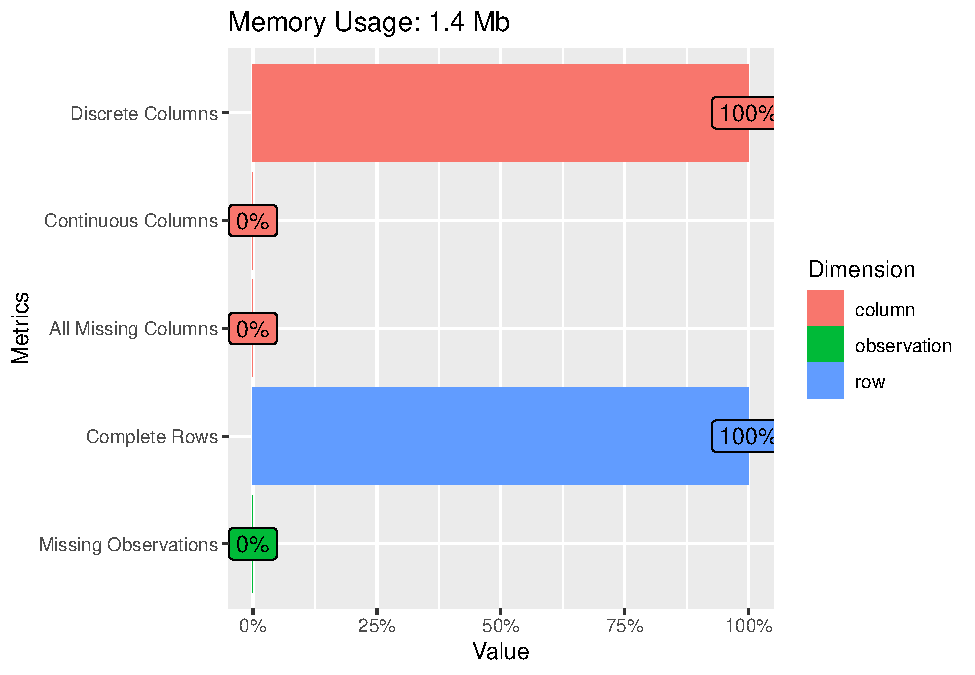
\includegraphics{Test_files/figure-latex/data exploration-1.pdf}

\begin{Shaded}
\begin{Highlighting}[]
\KeywordTok{plot_missing}\NormalTok{(mushroom_data)}
\end{Highlighting}
\end{Shaded}

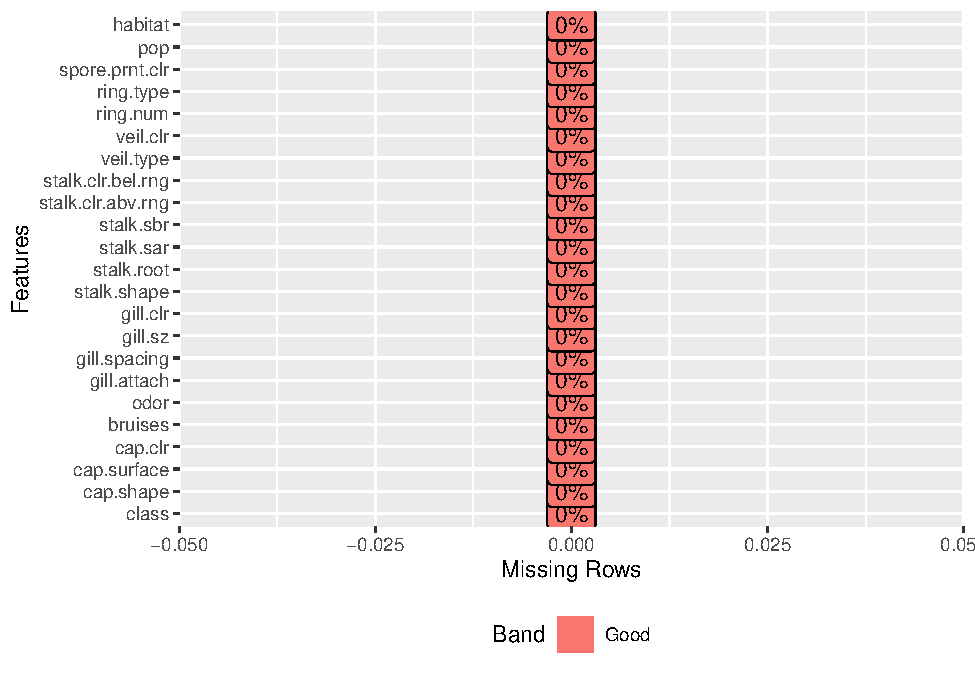
\includegraphics{Test_files/figure-latex/data exploration-2.pdf}

\begin{Shaded}
\begin{Highlighting}[]
\KeywordTok{plot_correlation}\NormalTok{(mushroom_data)}
\end{Highlighting}
\end{Shaded}

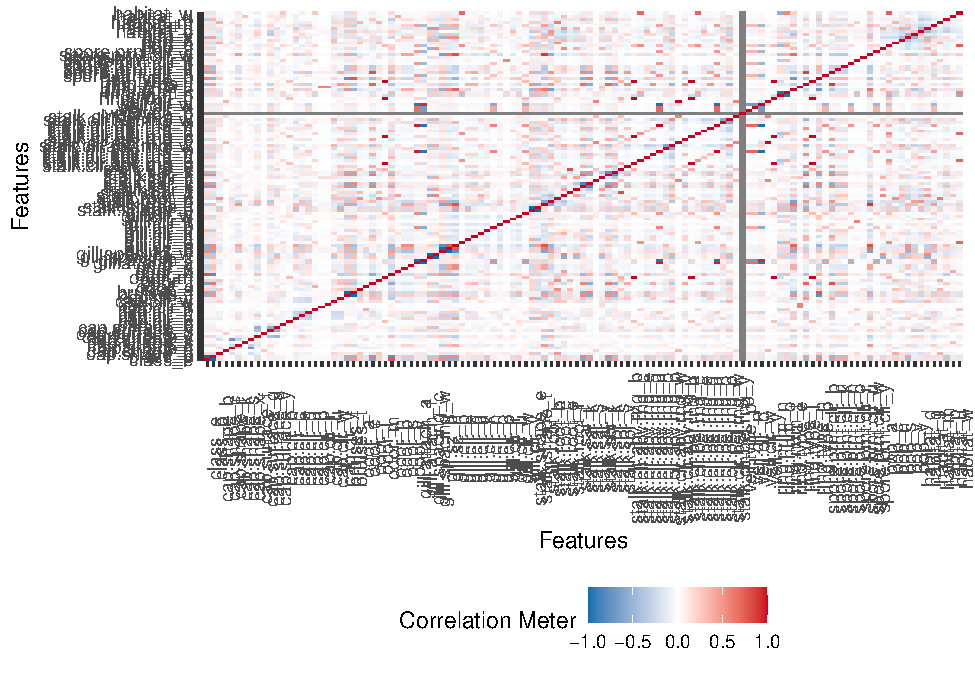
\includegraphics{Test_files/figure-latex/data exploration-3.pdf}

\begin{Shaded}
\begin{Highlighting}[]
\KeywordTok{str}\NormalTok{(mushroom_data)}
\end{Highlighting}
\end{Shaded}

\begin{verbatim}
## 'data.frame':    8124 obs. of  23 variables:
##  $ class            : chr  "p" "e" "e" "p" ...
##  $ cap.shape        : chr  "x" "x" "b" "x" ...
##  $ cap.surface      : chr  "s" "s" "s" "y" ...
##  $ cap.clr          : chr  "n" "y" "w" "w" ...
##  $ bruises          : chr  "t" "t" "t" "t" ...
##  $ odor             : chr  "p" "a" "l" "p" ...
##  $ gill.attach      : chr  "f" "f" "f" "f" ...
##  $ gill.spacing     : chr  "c" "c" "c" "c" ...
##  $ gill.sz          : chr  "n" "b" "b" "n" ...
##  $ gill.clr         : chr  "k" "k" "n" "n" ...
##  $ stalk.shape      : chr  "e" "e" "e" "e" ...
##  $ stalk.root       : chr  "e" "c" "c" "e" ...
##  $ stalk.sar        : chr  "s" "s" "s" "s" ...
##  $ stalk.sbr        : chr  "s" "s" "s" "s" ...
##  $ stalk.clr.abv.rng: chr  "w" "w" "w" "w" ...
##  $ stalk.clr.bel.rng: chr  "w" "w" "w" "w" ...
##  $ veil.type        : chr  "p" "p" "p" "p" ...
##  $ veil.clr         : chr  "w" "w" "w" "w" ...
##  $ ring.num         : chr  "o" "o" "o" "o" ...
##  $ ring.type        : chr  "p" "p" "p" "p" ...
##  $ spore.prnt.clr   : chr  "k" "n" "n" "k" ...
##  $ pop              : chr  "s" "n" "n" "s" ...
##  $ habitat          : chr  "u" "g" "m" "u" ...
\end{verbatim}

Above a few visuals show inspecting the data is quite difficult in its current state. All of the columns are read in as characters, which makes building visuals and getting a summary of the data quite difficult. The last command of str(mushroom\_data) does provide a small amount of information. The column class is the target variable to determine whether or not a mushroom is poisonous or not, and the veil.type column has only one level, or is a constant thus will not provide insight for the model and can be removed. The head function does show the stalk.root column having \enquote{?} in the data, which is a sign of missing data. To alleviate this problem the ? will be converted to \enquote{u} to give a label of unknown to the data.

\begin{Shaded}
\begin{Highlighting}[]
\NormalTok{shroom_dat <-}\StringTok{ }\KeywordTok{subset}\NormalTok{(mushroom_data, }\DataTypeTok{select =} \OperatorTok{-}\KeywordTok{c}\NormalTok{(}\StringTok{`}\DataTypeTok{veil.type}\StringTok{`}\NormalTok{))}
\KeywordTok{levels}\NormalTok{(shroom_dat}\OperatorTok{$}\StringTok{`}\DataTypeTok{stalk.root}\StringTok{`}\NormalTok{)[}\KeywordTok{levels}\NormalTok{(shroom_dat}\OperatorTok{$}\StringTok{`}\DataTypeTok{stalk.root}\StringTok{`}\NormalTok{)}\OperatorTok{==}\StringTok{"?"}\NormalTok{] <-}\StringTok{ "u"} \CommentTok{#converts missing data to "unknown"}

\NormalTok{shroom_dat}\OperatorTok{$}\NormalTok{class <-}\StringTok{ }\KeywordTok{as.factor}\NormalTok{(shroom_dat}\OperatorTok{$}\NormalTok{class)}
\KeywordTok{str}\NormalTok{(shroom_dat)}
\end{Highlighting}
\end{Shaded}

\begin{verbatim}
## 'data.frame':    8124 obs. of  22 variables:
##  $ class            : Factor w/ 2 levels "e","p": 2 1 1 2 1 1 1 1 2 1 ...
##  $ cap.shape        : chr  "x" "x" "b" "x" ...
##  $ cap.surface      : chr  "s" "s" "s" "y" ...
##  $ cap.clr          : chr  "n" "y" "w" "w" ...
##  $ bruises          : chr  "t" "t" "t" "t" ...
##  $ odor             : chr  "p" "a" "l" "p" ...
##  $ gill.attach      : chr  "f" "f" "f" "f" ...
##  $ gill.spacing     : chr  "c" "c" "c" "c" ...
##  $ gill.sz          : chr  "n" "b" "b" "n" ...
##  $ gill.clr         : chr  "k" "k" "n" "n" ...
##  $ stalk.shape      : chr  "e" "e" "e" "e" ...
##  $ stalk.root       : chr  "e" "c" "c" "e" ...
##   ..- attr(*, "levels")= chr(0) 
##  $ stalk.sar        : chr  "s" "s" "s" "s" ...
##  $ stalk.sbr        : chr  "s" "s" "s" "s" ...
##  $ stalk.clr.abv.rng: chr  "w" "w" "w" "w" ...
##  $ stalk.clr.bel.rng: chr  "w" "w" "w" "w" ...
##  $ veil.clr         : chr  "w" "w" "w" "w" ...
##  $ ring.num         : chr  "o" "o" "o" "o" ...
##  $ ring.type        : chr  "p" "p" "p" "p" ...
##  $ spore.prnt.clr   : chr  "k" "n" "n" "k" ...
##  $ pop              : chr  "s" "n" "n" "s" ...
##  $ habitat          : chr  "u" "g" "m" "u" ...
\end{verbatim}

\hypertarget{svm-model}{%
\subsection{SVM Model}\label{svm-model}}

The data is ready to be split and models are ready to be applied. The first model that will be used is the Support Vector Machine, which creates planes based off features to classify the data to either \enquote{edible} or \enquote{poisonous}. For curiosity sake, all four types of the SVM models will be applied to compare how they impact results. SVM models traditionally require numeric data in order for them to function; however, thanks to some help from the e1071 library the data is interpreted as numeric

\begin{Shaded}
\begin{Highlighting}[]
\NormalTok{idx <-}\StringTok{ }\KeywordTok{createDataPartition}\NormalTok{(shroom_dat}\OperatorTok{$}\NormalTok{class, }\DataTypeTok{p=}\FloatTok{0.7}\NormalTok{, }\DataTypeTok{list=}\OtherTok{FALSE}\NormalTok{) }\CommentTok{#creates index to split data}

\NormalTok{shroom_train <-}\StringTok{ }\NormalTok{shroom_dat[idx,]}
\NormalTok{shroom_test <-}\StringTok{ }\NormalTok{shroom_dat[}\OperatorTok{-}\NormalTok{idx,] }

\NormalTok{svm_linear <-}\StringTok{ }\KeywordTok{svm}\NormalTok{(class}\OperatorTok{~}\NormalTok{., }\DataTypeTok{data=}\NormalTok{shroom_train, }\DataTypeTok{type=}\StringTok{'C-classification'}\NormalTok{, }\DataTypeTok{kernel=}\StringTok{'linear'}\NormalTok{) }\CommentTok{# applies svm with a linear fit}
\NormalTok{shroom_lin_pred <-}\StringTok{ }\KeywordTok{predict}\NormalTok{(svm_linear, shroom_test)}
\NormalTok{svm_radial <-}\StringTok{ }\KeywordTok{svm}\NormalTok{(class}\OperatorTok{~}\NormalTok{., }\DataTypeTok{data=}\NormalTok{shroom_train, }\DataTypeTok{type=}\StringTok{'C-classification'}\NormalTok{, }\DataTypeTok{kernel=}\StringTok{'radial'}\NormalTok{) }\CommentTok{# applies svm with a radial fit}
\NormalTok{shroom_rad_pred <-}\StringTok{ }\KeywordTok{predict}\NormalTok{(svm_radial, shroom_test)}
\NormalTok{svm_poly <-}\StringTok{ }\KeywordTok{svm}\NormalTok{(class}\OperatorTok{~}\NormalTok{., }\DataTypeTok{data=}\NormalTok{shroom_train, }\DataTypeTok{type=}\StringTok{'C-classification'}\NormalTok{, }\DataTypeTok{kernel=}\StringTok{'polynomial'}\NormalTok{) }\CommentTok{# applies svm with a polynomial fit}
\NormalTok{shroom_poly_pred <-}\StringTok{ }\KeywordTok{predict}\NormalTok{(svm_poly, shroom_test)}
\NormalTok{svm_sigmoid <-}\StringTok{ }\KeywordTok{svm}\NormalTok{(class}\OperatorTok{~}\NormalTok{., }\DataTypeTok{data=}\NormalTok{shroom_train, }\DataTypeTok{type=}\StringTok{'C-classification'}\NormalTok{, }\DataTypeTok{kernel=}\StringTok{'sigmoid'}\NormalTok{) }\CommentTok{# applies svm with a sigmoid fit}
\NormalTok{shroom_sig_pred <-}\StringTok{ }\KeywordTok{predict}\NormalTok{(svm_sigmoid, shroom_test)}

\KeywordTok{confusionMatrix}\NormalTok{(shroom_lin_pred, shroom_test}\OperatorTok{$}\NormalTok{class)}\OperatorTok{$}\NormalTok{table }
\end{Highlighting}
\end{Shaded}

\begin{verbatim}
##           Reference
## Prediction    e    p
##          e 1262    0
##          p    0 1174
\end{verbatim}

\begin{Shaded}
\begin{Highlighting}[]
\KeywordTok{confusionMatrix}\NormalTok{(shroom_rad_pred, shroom_test}\OperatorTok{$}\NormalTok{class)}\OperatorTok{$}\NormalTok{table}
\end{Highlighting}
\end{Shaded}

\begin{verbatim}
##           Reference
## Prediction    e    p
##          e 1262    3
##          p    0 1171
\end{verbatim}

\begin{Shaded}
\begin{Highlighting}[]
\KeywordTok{confusionMatrix}\NormalTok{(shroom_poly_pred, shroom_test}\OperatorTok{$}\NormalTok{class)}\OperatorTok{$}\NormalTok{table}
\end{Highlighting}
\end{Shaded}

\begin{verbatim}
##           Reference
## Prediction    e    p
##          e 1248  148
##          p   14 1026
\end{verbatim}

\begin{Shaded}
\begin{Highlighting}[]
\KeywordTok{confusionMatrix}\NormalTok{(shroom_sig_pred, shroom_test}\OperatorTok{$}\NormalTok{class)}\OperatorTok{$}\NormalTok{table}
\end{Highlighting}
\end{Shaded}

\begin{verbatim}
##           Reference
## Prediction    e    p
##          e 1262   30
##          p    0 1144
\end{verbatim}

\newpage

\hypertarget{references}{%
\section{References}\label{references}}

Günther, F., and Fritsch, S. (2010). neuralnet: Training of neural networks. The R journal, 2(1), 30-38.

Yu-Wei, C. (2015). Machine Learning with R Cookbook. Packt Publishing.

Lantz, B. (2015). Machine Learning with R: Expert Techniques for Predictive Modeling to Solve All Your Data Analysis Problems: Vol. Second edition. Packt Publishing.

\begingroup
\setlength{\parindent}{-0.5in}
\setlength{\leftskip}{0.5in}

\hypertarget{refs}{}

\endgroup


\end{document}
